\ifx\isEmbedded\undefined


\documentclass[11pt,a4paper]{article}
\usepackage[utf8]{inputenc}		% LaTeX, comprend les accents !
\usepackage[T1]{fontenc}
\usepackage{natbib}	
%\usepackage[square,sort&compress,sectionbib]{natbib}		% Doit être chargé avant babel      
\usepackage[frenchb,english]{babel}
\usepackage{lmodern}
\usepackage{amsmath,amssymb, amsthm}
\usepackage{a4wide}
\usepackage[capposition=top]{floatrow}
\usepackage{verbatim}
\usepackage{float}
\usepackage{placeins}
\usepackage{flafter}
\usepackage{longtable}
\usepackage{pdflscape}
\usepackage{rotating}
\usepackage{hhline}
\usepackage{multirow}
\usepackage{booktabs}
\usepackage[pdftex,pdfborder={0 0 0},colorlinks=true,linkcolor=blue,urlcolor=blue,citecolor=blue,bookmarksopen=true]{hyperref}
\usepackage{eurosym}
\usepackage{breakcites}
\usepackage[autostyle]{csquotes}
%\usepackage{datetime}
\usepackage{natbib}
\usepackage{setspace}
\usepackage{lscape}
\usepackage[usenames]{color}
\usepackage{indentfirst}

\usepackage{url}
\usepackage{enumitem}
\usepackage{multirow}
\usepackage{subcaption}
\usepackage[justification=centering]{caption}
\bibliographystyle{agsm}

\usepackage{array}

\begin{document}

\else \fi
%%%%%%%%%%%%%%%%%%%%%%%%%%%%%%%%%%%%%%%%%%%%%%%%%%%%%%%%%%%%%%%%%%%%%%%%%%%%%%%%%%%%%%%%%%%%%%%%%%%%%%%%%%%%%%



\section{L'analyse des données: résultats préliminaires}

En amont du choix de modélisation, il est nécessaire de documenter la variabilité individuelle dans les différents phénomènes que l'on souhaite modéliser. Par rapport à des trajectoires totalement déterministes, l'aléa peut venir (i) de la durée passée dans l'échelon (ii) de la possibilité de changement de grade en milieu de grille et (iii) le grade de destination quand on observe un changement de grade. 

\subsection{Analyser la vitesse de progression: un travail de complétion nécessaire}

Nous regroupons les points (i) et (ii) autour de la notion de vitesse de progression de carrière: vitesse de progression dans l'échelon et d'un grade à l'autre. Nous voudrions comparer la durée passée dans un échelon ou un grade donné pour un individu donné, à la vitesse prévue par la grille d'une part, et à la durée observé pour le reste de la population d'autre part. Cela nécessite d'être en mesure de connaitre la durée passée dans le grade ou l'échelon à chaque date donnée, et donc un certain recul historique. 

Comme mentionné plus haut, la reconstitution de la trajectoire statutaire -- c'est-à-dire de l'échelon et du grade -- sur le passé (avant 2011) reste à affiner. Dès lors nous n'avons pu à ce stade documenter de manière précise ces éléments, pourtant centraux pour la modélisation de l'évolution de la rémunération. 


\subsection{Analyser les grades de destination: premiers résultats}

L'analyse des données sur les années 2011-2014 permet de documenter une autre question importante par rapport aux choix de modélisation: le grade de destination quand on observe un changement de grade pour un individu donné. L'approche adoptée est la suivante: pour chaque grade, nous considérons les années pour laquelle nous observons un changement de grade entre l'année $n$ et l'année $n+1$, et calculons les agrégats suivantes: 


\begin{itemize}[leftmargin=1cm ,parsep=0cm,itemsep=0cm,topsep=0cm] 
\item Le nombre de grades possibles en $n+1$
\item La proportion d'individus passant dans le grade le plus représenté en $n+1$, les deux plus représentés, les trois plus représentés, et les 5 plus représentés. 
\end{itemize}

Les moyennes sur l'ensemble de la population, pondérée ou non en fonction du nombre de transitions observées pour le grade considérée, sont présentées à la table \ref{means}. Même s'il existe un nombre élevé de transitions possibles en moyenne, la grande majorité des transitions se fait vers un petit nombres de grade possible. Ainsi par exemple 94\% des transitions observés se font vers les 3 destinations principales (propres à chaque grade). Ce constat est confirmé au graphique \ref{pct},

\begin{table}[ht]
\label{means}
\centering
\caption{Destinations en cas de changement de grade} 
\begin{tabular}{l|cc}
  \hline
 & Moyenne simple & Moyenne pondérée \\ 
  \hline
Nombre de destinations & 11.4 & 45.5 \\ 
  Part de la destination majoritaire   & 66.1 \% & 58.8 \%  \\ 
  Part des 2 destinations majoritaires & 87.4 \% & 87.0 \% \\ 
  Part des 3 destinations majoritaires & 93.6 \% & 92.8 \% \\ 
  Part des 5 destinations majoritaires & 97.5 \% & 96.1 \% \\ 
   \hline
\end{tabular}
\end{table}

\begin{figure}[t]
  \label{pct}
\caption{Distribution de la proportion de transitions vers les destinations principales}
\vspace{-0.1cm}
\centering
  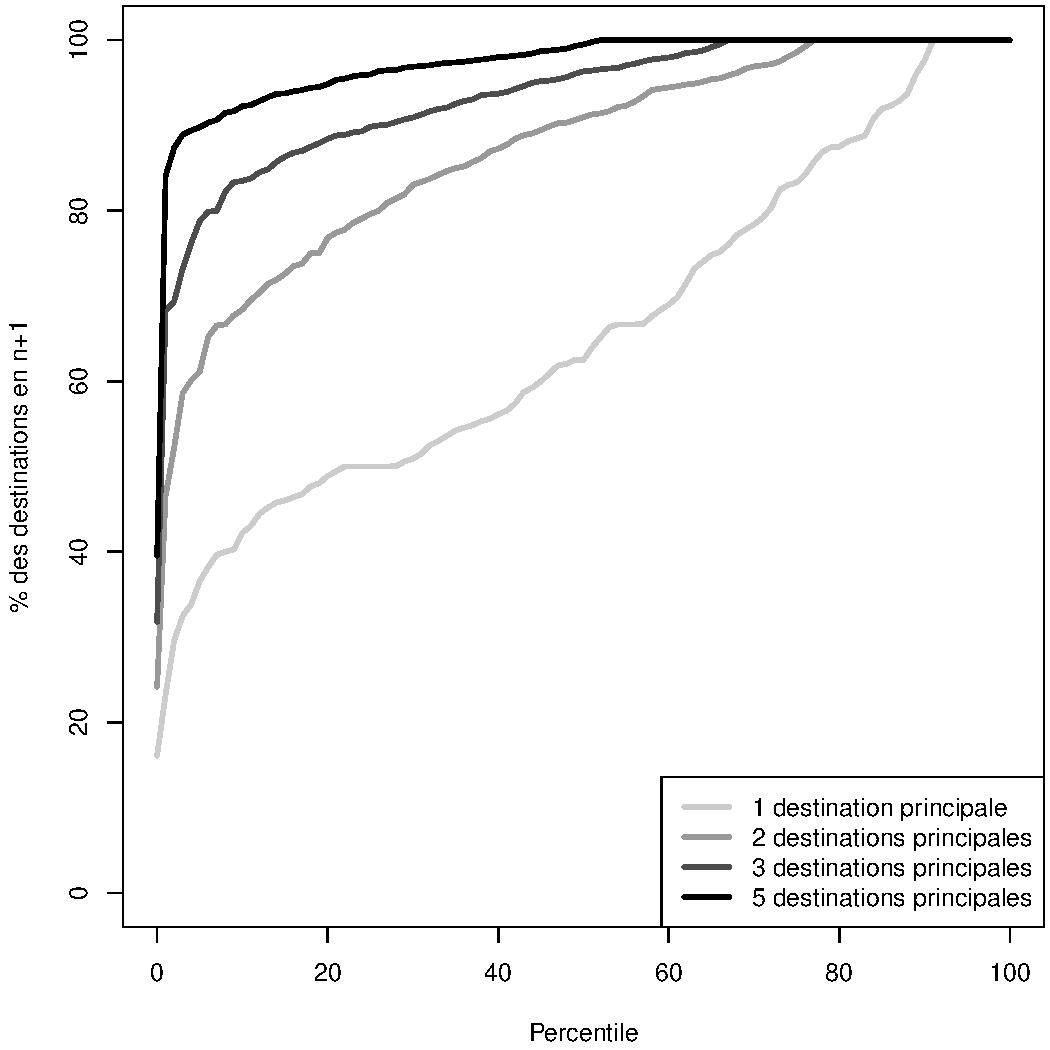
\includegraphics[width=0.7\linewidth]{../../../fonction-publique/fonction_publique/bordeaux/results/pct.pdf}
\vspace{0.1cm}  
\begin{minipage}{12cm}%
\small \textsc{Lecture:} Pour environ 50 \% des grades, les 5 destinations les plus fréquentes représentent 100 \% des transitions observées.  
 \end{minipage}%
\end{figure}

En se concentrant sur les grades les plus représentés\footnote{TTH1 adjoint technique de 2eme classe, TAJ1 adjoint administratif de 2ème classe, 3001 aide soignant classe normale, 2432 infirmier de classe normale}
pour les générations 1970-1979, il apparaît (voir la table \ref{tab:destination}) que l'écrasante majorité des transitions se fait dans le garde immédiatement supérieur quand elles ne se font pas vers un non-grade.
\begin{table}[htbp]
    \label{tab:destination}
    \centering
    \caption{Destinations en cas de changement de grade (avec grade vide)} 
    \begin{tabular}{llrr}
\toprule
initial & destination &  nombre & part \\
\midrule
        &      autres &   90946 & 68 \% \\
        &        TTH1 &   21439 & 16 \% \\
        &        3001 &   10797 &  8 \% \\
        &        TAJ1 &   10137 &  8 \% \\
   TTH1 &             &    8416 & 43 \% \\
   TTH1 &        TTH2 &    8231 & 42 \% \\
   TTH1 &      autres &    2490 & 13 \% \\
   TTH1 &        TMD1 &     431 &  2 \% \\
   3001 &             &    5900 & 47 \% \\
   3001 &        3002 &    5389 & 43 \% \\
   3001 &      autres &     795 &  6 \% \\
   3001 &        2432 &     533 &  4 \% \\
   TAJ1 &        TAJ2 &    6346 & 48 \% \\
   TAJ1 &             &    5511 & 42 \% \\
   TAJ1 &      autres &     878 &  7 \% \\
   TAJ1 &        TAR1 &     396 &  3 \% \\
\bottomrule
\end{tabular}

\end{table}

En se limitant aux carrières ne présentant pas d'épisode ou la grade n'est pas renseigné, il apparaît que la destination est dans près de 80 \% des cas le grade immédiatement supérieur (passage à la classe supérieure) dans le corps ou le cadre d'emploi (voir la table \ref{tab:destination}).       

\begin{table}[htbp]
    \label{tab:purged_destination}
    \centering
    \caption{Destinations en cas de changement de grade (carrières sans grade vide)} 
    \begin{tabular}{llrr}
\toprule
initial & destination &  nombre & part \\
\midrule
   TTH1 &        TTH2 &    7479 & 75 \% \\
   TTH1 &      autres &    1736 & 17 \% \\
   TTH1 &        TMD1 &     383 &  4 \% \\
   TTH1 &        TAJ1 &     362 &  4 \% \\
   3001 &        3002 &    5207 & 82 \% \\
   3001 &        2432 &     510 &  8 \% \\
   3001 &      autres &     505 &  8 \% \\
   3001 &        3121 &     134 &  2 \% \\
   TAJ1 &        TAJ2 &    5581 & 84 \% \\
   TAJ1 &      autres &     446 &  7 \% \\
   TAJ1 &        TAR1 &     345 &  5 \% \\
   TAJ1 &        TTH1 &     278 &  4 \% \\
   2432 &        2753 &    2645 & 79 \% \\
   2432 &      autres &     416 & 12 \% \\
   2432 &        2801 &     188 &  6 \% \\
   2432 &        1801 &      82 &  2 \% \\
\bottomrule
\end{tabular}

\end{table}

Questions à discuter
\begin{enumerate}[leftmargin=1cm ,parsep=0cm,itemsep=0cm,topsep=0cm] 
\item Quel statut des transitions vers une missing value? Problème de donnée ou disponibilité ou sortie de la FP? Module rémunération, carrière ou affiliation? 
\end{enumerate}



%%%%%%%%%%%%%%%%%%%%%%%%%%%%%%%%%%%%%%%%%%%%%%%%%%%%%%%%%%%%%%%%%%%%%%%%%%%%

\ifx\isEmbedded\undefined
\newpage
\bibliographystyle{../../Divers/myagsm} 
\bibliography{../../Divers/biblio_these}
\end{document}
\else \fi

